\subsection{Versuchsaufbau}
\label{sec:Versuchsaufbau}
Der prinzipille Versuchsaufbau ist in Abbildung \ref{fig:aufbau} dargestellt.
Die im Zählrohr am Anodendraht gesammelte Ladung $Q$ fließt über einen Widerstand $R$ ab und erzeugt an diesem einen Spannungsimpuls. Über einen Kondensator $C$ wird dieser ausgekoppelt, mittels eines Verstärkers verstärkt und an ein Zählgerät sowie ein Oszilloskop weitergeleitet.\\
Das Zählgerät hat einen eingebauten Timer, welcher es ermöglicht, Impulse innerhalb eines festen Zeitintervalls zu zählen (Im vorliegenden Versuch: $\SI{1}{\minute}$).
Die registrierten Impulse können außerdem auf dem Schirm des Oszilloskops analysiert werden.\\
Der prinzipielle Aufbau des Geiger-Müller-Zählrohrs ist in Abbildung \ref{fig:geige} dargestellt.
Das Geiger-Müller-Zählrohr besteht aus einem Kathodenzylinder sowie einem mittig darin angebrachten Anodendraht, welcher über einen Isolator aus dem Geiger-Müller-Zählrohr herausgeführt wird.
Über das Anlegen einer äußeren Spannung liegt im Geiger-Müller-Zählrohr ein radialsymetrisches elektrisches Feld vor.\\
Der Hohlraum im Geiger-Müller-Zählrohr ist mit einem Gasgemisch gefüllt.
Das Eintrittsfenster des Zählrohrs besteht aus Mylar, welches zugleich dem Unterdruck im Zählrohr standhält, als auch durchlässig für auftreffende Teilchen ist.

\begin{figure}
  \centering
  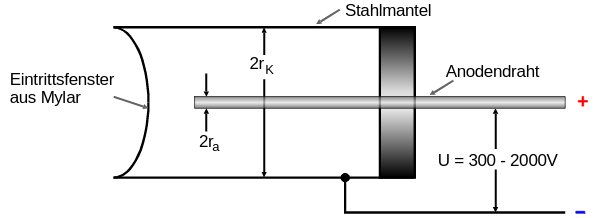
\includegraphics[width=0.8\textwidth]{Bilder/endfenster.png}
  \caption{Prinzipieller Aufbau eines Geiger-Müller-Zählrohrs. \cite{Anleitung}}
  \label{fig:geige}
\end{figure}



\begin{figure}
  \centering
  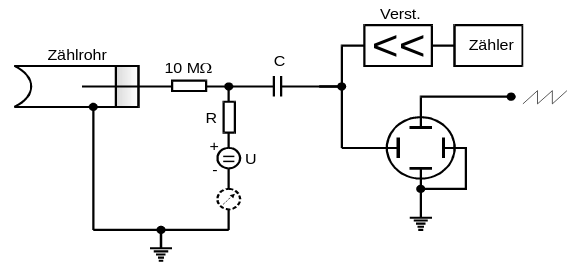
\includegraphics[width=0.8\textwidth]{Bilder/aufbau.png}
  \caption{Prinzipieller Versuchsaufbau zur Untersuchung des Geiger-Müller-Zählrohrs. \cite{Anleitung}}
  \label{fig:aufbau}
\end{figure}
